To begin identifying an appropriate development methodology, it is necessary to understand the project requirements. The project requirements are determined over a number of meetings with the primary stakeholders. These meetings discuss the minimum requirements and the features that are going to be implemented on the project. A more detailed reference on all the requirements is discussed in the previous section.

The next step is deciding the methodology that will be used. Since we are looking for iterative and incremental development, Agile Software Development Methodology will be followed. This also enables time-boxed iterative approach. Agile methods are focused on different aspects of the software development life cycle. Two of the most well known agile methodologies are Scrum and XP.

Scrum is a project management agile framework. It's use focuses more on the management of software development projects. The term is named after the scrum (or scrummage) formation in rugby, which is used to restart the game after an event that causes play to stop. There are some core roles in Scrum. Firstly there is the ScrumMaster, who maintains the scrum process and keeps everyone focused on their tasks, secondly the Product Owner represents the client and finally the team, a group building the product. The product is completed in many one to four week iterations, or sprints. Before each sprint, a planning meeting is held to define which features will be implemented during that sprint. There are also meetings that occur daily and last 15 minutes. These meetings are called SCRUM meetings where each member answers three questions: 1) What have you done since yesterday?, 2)What are you planning to do today?, 3)Any impediments/stumbling blocks?

Similarly, XP (Extreme Programming) is an agile methodology which focuses on the values of simplicity, communication, feedback, and courage. XP is designed for small, co-located teams aiming to get quality and productivity as high as possible. It does this through the use of rich, short, informal communication paths with emphasis on skill, discipline, and understanding at the personal level, minimizing all intermediate work products. XP includes within its definition a selection of practises that the team members need to learn. Those techniques are as follows:

\begin{itemize}
\item The planning game and the stand-up meeting where the team uses a simple planning form in order to decide what to do next and it gives deadlines in each part of the project. 
\item The test-driven development along with the refactoring where the programmers produce code which include tests. At all times, they are to keep the overall design as simple as they can and the code as clear as they can. This constant refactoring is possible because of the extensive unit test suites in place.
\item The pair programming and the continuous integration where the programmers work together in pairs and all the team works together all the time. They also keep the system fully integrated at all times. 
\end{itemize}

As this is a college project and tight time constraints apply, it is quite difficult to follow a particular methodology. Scrum focuses on the management side of the project whereas XP focuses more on the actual programming practices. It is more preferable if various elements from both methodologies will be used since they address different areas and complement each other.

We decided to focus on managing the software project using the scrum approach and adopt it's characteristics that suit our own project. The team is composed by six students each one assigned with various tasks every week. Weekly meetings are also planned in order to organise the division of work and for the team to get up to speed with what every one is doing or completed. An agenda is stored in a document that holds the content and matters which the team discusses in each meeting.

To make the production more effective and faster, an online collaboration tool called "Trello" is used. This tool gives access to a visual board and displays all the required short-term or long-term tasks which are represented as cards with various labels and priorities. This board is very similar to the scrum board as shown in the following pictures:

\begin{figure}[here]
\begin{minipage}{\textwidth}
\begin{center}
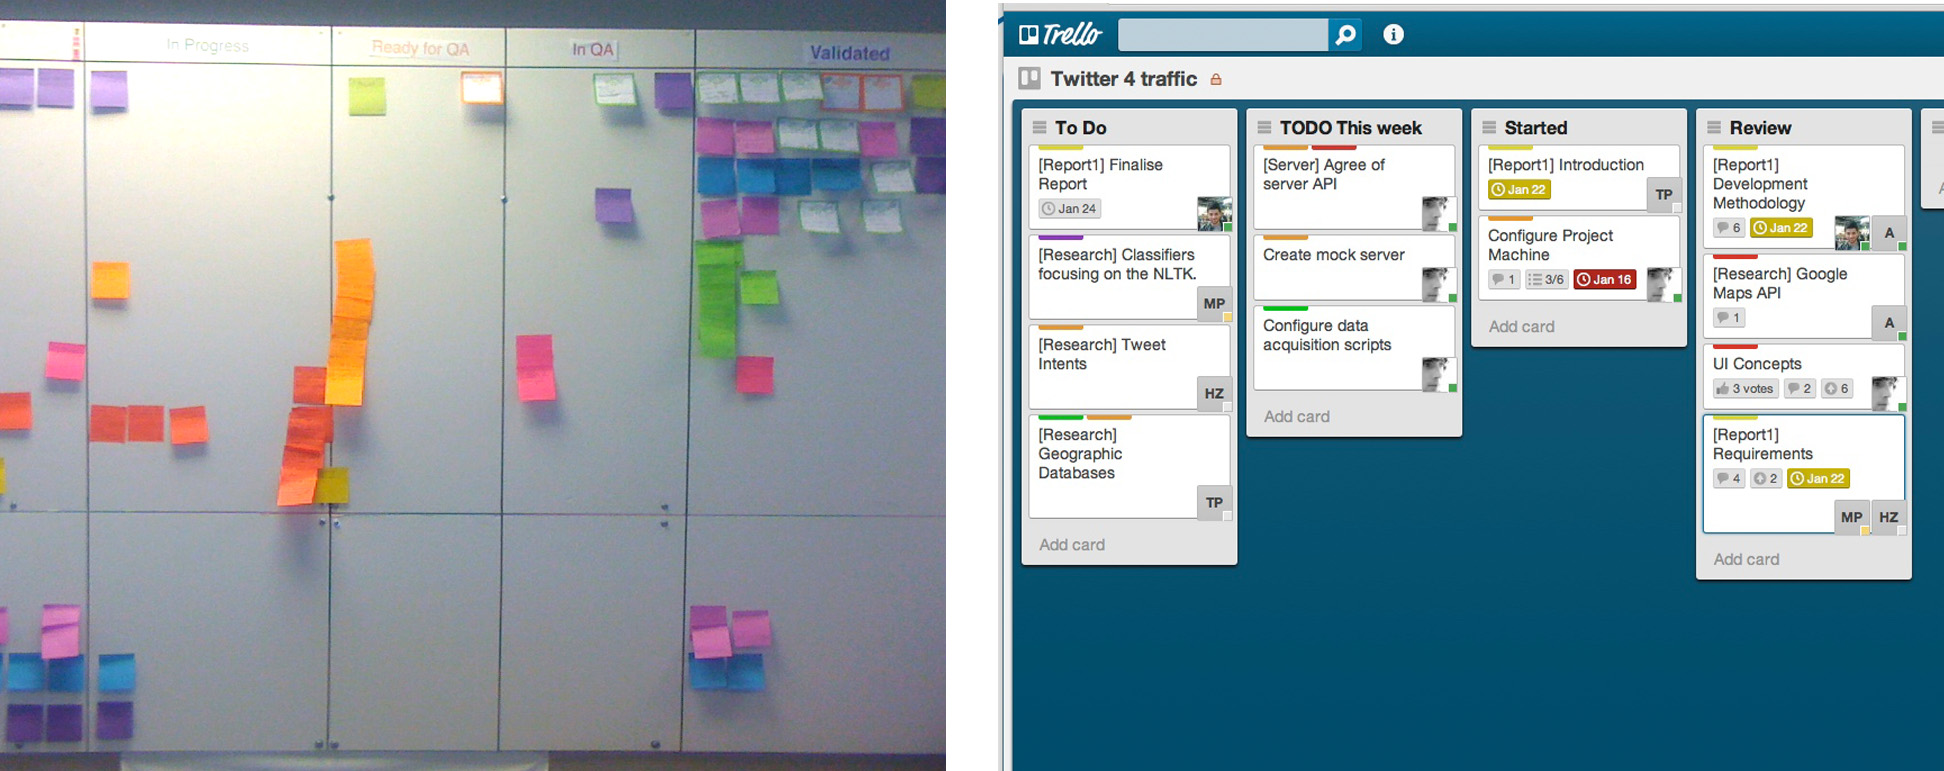
\includegraphics[width=0.95\textwidth]{images/scrumboard.jpg}
\end{center}
\vspace{-20pt}
\caption[Caption for LOF]{Scrum Board and Trello\footnotemark}
\end{minipage} 
\end{figure}
\footnotetext{Left: CC Drew Stephens flickr.com/photos/dinomite/3695570625, Right: (C)Trello.com}


We also decided to adopt several techniques from the XP, which will help us improve the programming process. The first practise we decided to use is pair programming, having two programmers work alongside on the same code. At any time, those two programmers sitting together may change any line of code in the system. Any time the two find a section of code that appears hard to understand or overly complex, they are to revise it, constantly simplifying and improving it. This technique improves the code quality and the team focus. Furthermore, several tests will be added in our code-base, keeping a test-driven development . However because of the nature of the project being partly research based and the results being quite subjective, it is difficult to test effectively. Hence, the development of the mobile application will be a TDD whereas for the server development we won't be able to follow strictly the TDD.\cite{Cockburn}

For the division of work amongst the project, more flexibility will be achieved by maximising the use of the members previous experience, but also keeping everyone interested. A balanced division has been decided where two members of the team will focus on the mobile application, two on the server side and the rest will move between those two tasks as necessary. However these movements have to be kept to the minimum because we are well aware of the Brook's Law which emphasizes that adding manpower to a late software project makes it later.\cite{Brooks}

To facility parallel development, the server API will be mocked-up and will produce a fixed data set in the desired format that the android applications can handle. That way, those developing the mobile application can work independently from those working on the server. One person on the team is designated as the team "coach". This person reviews with the team members their use of the key practices: use of pair programming and testing,keeping design simple, communicating, and so on.

As regards the actual design of the project there are multiple aspects. The first one is the mobile application that will act as the front-end of the system. For the user interface, some Lo-Fi layouts will be drawn in paper in order to have a general idea of how the interface is going to look like. The relative data will be retrieved in a structured form that will be the same for the server and the mobile application. The second aspect is the server implementation. A project machine will be used for the server, where traffic feeds from TFL and Twitter will be retrieved in XML format and stored in a database.
